% fig_7_1_contributions_future.tex
% Mind map: contributions radiating above, future directions below
% Compile: pdflatex fig_7_1_contributions_future.tex
\documentclass[tikz,border=5pt]{standalone}

\usepackage[T1]{fontenc}
\usepackage[utf8]{inputenc}
\usepackage{amsmath,amssymb}
\usepackage{tikz}
\usetikzlibrary{arrows.meta, positioning, shapes.geometric, calc, decorations.markings}

% ── Color palette ──────────────────────────────────────────────────
\definecolor{centerColor}{HTML}{1565C0}
\definecolor{centerFill}{HTML}{E3F2FD}
\definecolor{contribGreen}{HTML}{2E7D32}
\definecolor{contribGreenFill}{HTML}{E8F5E9}
\definecolor{futureOrange}{HTML}{E65100}
\definecolor{futureOrangeFill}{HTML}{FFF3E0}
\definecolor{arrowGray}{HTML}{546E7A}
\definecolor{labelGray}{HTML}{455A64}

\begin{document}
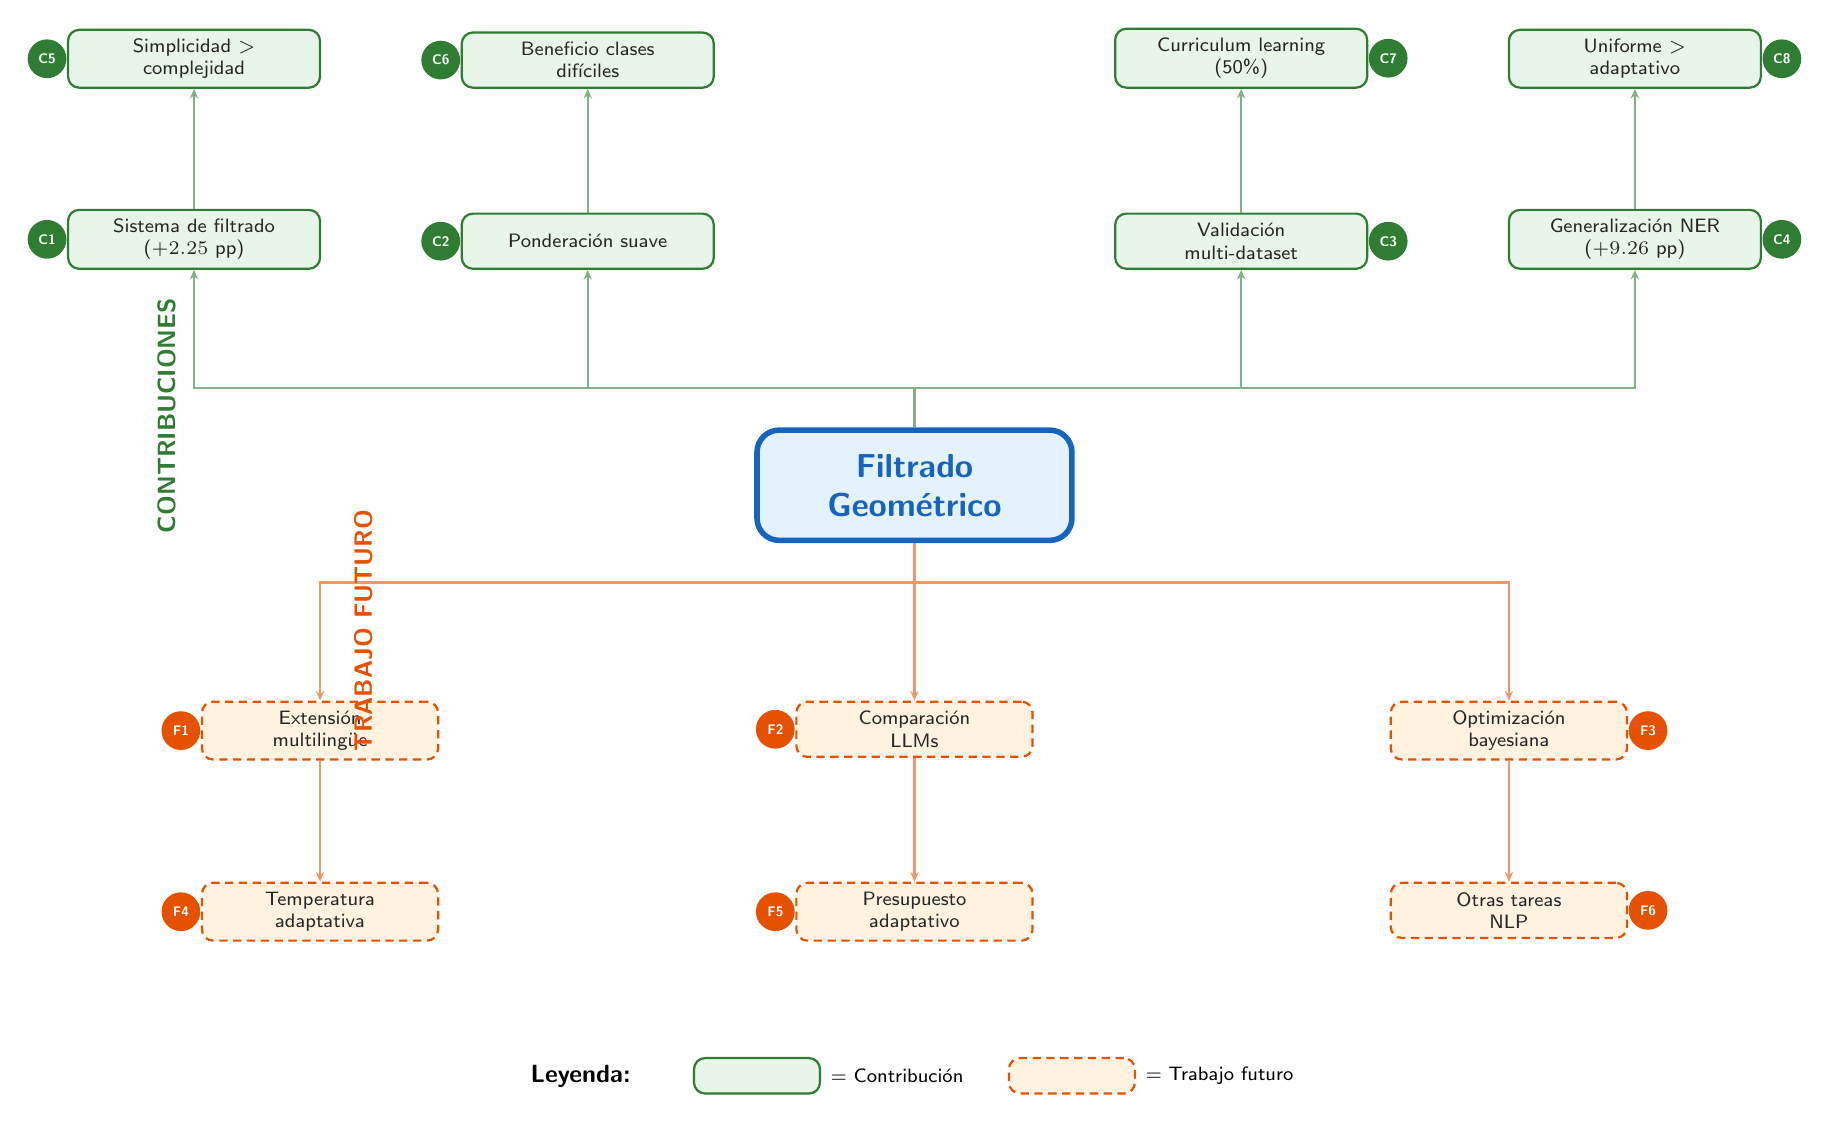
\begin{tikzpicture}[
    % ── shared styles ───────────────────────────────────────────────
    center node/.style={
        rectangle, rounded corners=8pt,
        fill=centerFill, draw=centerColor, line width=2pt,
        font=\sffamily\large\bfseries, text=centerColor,
        minimum height=1.4cm, minimum width=4.0cm,
        align=center,
    },
    contrib/.style={
        rectangle, rounded corners=4pt,
        fill=contribGreenFill, draw=contribGreen, thick,
        font=\sffamily\scriptsize, text=black!85,
        minimum height=0.7cm, minimum width=3.2cm,
        align=center,
    },
    contrib id/.style={
        circle, fill=contribGreen, text=white,
        font=\sffamily\tiny\bfseries,
        inner sep=0pt, minimum size=14pt,
    },
    future/.style={
        rectangle, rounded corners=4pt,
        fill=futureOrangeFill, draw=futureOrange, thick, densely dashed,
        font=\sffamily\scriptsize, text=black!85,
        minimum height=0.7cm, minimum width=3.0cm,
        align=center,
    },
    future id/.style={
        circle, fill=futureOrange, text=white,
        font=\sffamily\tiny\bfseries,
        inner sep=0pt, minimum size=14pt,
    },
    conn up/.style={
        -{Stealth[length=3.5pt,width=3pt]},
        contribGreen!60, line width=0.9pt,
    },
    conn down/.style={
        -{Stealth[length=3.5pt,width=3pt]},
        futureOrange!60, line width=0.9pt,
    },
]

% =============================================================
%  CENTER NODE
% =============================================================
\node[center node] (center) at (0, 0) {Filtrado\\Geom\'{e}trico};

% =============================================================
%  CONTRIBUTIONS (C1--C8) -- radiating above
% =============================================================

% Row 1 (closest to center): C1, C2, C3, C4
\node[contrib, above left=2.0cm and 5.5cm of center] (c1)
    {Sistema de filtrado\\($+2.25$ pp)};
\node[contrib id, anchor=east] at (c1.west) {C1};

\node[contrib, above left=2.0cm and 0.5cm of center] (c2)
    {Ponderaci\'{o}n suave};
\node[contrib id, anchor=east] at (c2.west) {C2};

\node[contrib, above right=2.0cm and 0.5cm of center] (c3)
    {Validaci\'{o}n\\multi-dataset};
\node[contrib id, anchor=west] at (c3.east) {C3};

\node[contrib, above right=2.0cm and 5.5cm of center] (c4)
    {Generalizaci\'{o}n NER\\($+9.26$ pp)};
\node[contrib id, anchor=west] at (c4.east) {C4};

% Row 2 (further from center): C5, C6, C7, C8
\node[contrib, above left=4.3cm and 5.5cm of center] (c5)
    {Simplicidad $>$\\complejidad};
\node[contrib id, anchor=east] at (c5.west) {C5};

\node[contrib, above left=4.3cm and 0.5cm of center] (c6)
    {Beneficio clases\\dif\'{i}ciles};
\node[contrib id, anchor=east] at (c6.west) {C6};

\node[contrib, above right=4.3cm and 0.5cm of center] (c7)
    {Curriculum learning\\(50\%)};
\node[contrib id, anchor=west] at (c7.east) {C7};

\node[contrib, above right=4.3cm and 5.5cm of center] (c8)
    {Uniforme $>$\\adaptativo};
\node[contrib id, anchor=west] at (c8.east) {C8};

% Connection lines (center -> contributions)
\draw[conn up] (center.north) -- ++(0,0.5) -| (c1.south);
\draw[conn up] (center.north) -- ++(0,0.5) -| (c2.south);
\draw[conn up] (center.north) -- ++(0,0.5) -| (c3.south);
\draw[conn up] (center.north) -- ++(0,0.5) -| (c4.south);

\draw[conn up] (c1.north) -- (c5.south);
\draw[conn up] (c2.north) -- (c6.south);
\draw[conn up] (c3.north) -- (c7.south);
\draw[conn up] (c4.north) -- (c8.south);

% =============================================================
%  FUTURE DIRECTIONS (F1--F6) -- radiating below
% =============================================================

% Row 1 (closest to center): F1, F2, F3
\node[future, below left=2.0cm and 4.0cm of center] (f1)
    {Extensi\'{o}n\\multiling\"{u}e};
\node[future id, anchor=east] at (f1.west) {F1};

\node[future, below=2.0cm of center] (f2)
    {Comparaci\'{o}n\\LLMs};
\node[future id, anchor=east] at (f2.west) {F2};

\node[future, below right=2.0cm and 4.0cm of center] (f3)
    {Optimizaci\'{o}n\\bayesiana};
\node[future id, anchor=west] at (f3.east) {F3};

% Row 2 (further from center): F4, F5, F6
\node[future, below left=4.3cm and 4.0cm of center] (f4)
    {Temperatura\\adaptativa};
\node[future id, anchor=east] at (f4.west) {F4};

\node[future, below=4.3cm of center] (f5)
    {Presupuesto\\adaptativo};
\node[future id, anchor=east] at (f5.west) {F5};

\node[future, below right=4.3cm and 4.0cm of center] (f6)
    {Otras tareas\\NLP};
\node[future id, anchor=west] at (f6.east) {F6};

% Connection lines (center -> future)
\draw[conn down] (center.south) -- ++(0,-0.5) -| (f1.north);
\draw[conn down] (center.south) -- ++(0,-0.5) -| (f2.north);
\draw[conn down] (center.south) -- ++(0,-0.5) -| (f3.north);

\draw[conn down] (f1.south) -- (f4.north);
\draw[conn down] (f2.south) -- (f5.north);
\draw[conn down] (f3.south) -- (f6.north);

% =============================================================
%  Section labels
% =============================================================
\node[font=\sffamily\small\bfseries, text=contribGreen, anchor=east,
      rotate=90] at (-9.5, 2.5) {CONTRIBUCIONES};

\node[font=\sffamily\small\bfseries, text=futureOrange, anchor=west,
      rotate=90] at (-7.0, -3.5) {TRABAJO FUTURO};

% =============================================================
%  Legend
% =============================================================
\begin{scope}[shift={(-5.0, -7.5)}]
  \node[font=\sffamily\small\bfseries, anchor=west] at (0, 0) {Leyenda:};

  \node[contrib, minimum width=1.6cm, minimum height=0.45cm] (legC) at (3.0, 0) {};
  \node[font=\sffamily\scriptsize, anchor=west] at (legC.east) { = Contribuci\'{o}n};

  \node[future, minimum width=1.6cm, minimum height=0.45cm] (legF) at (7.0, 0) {};
  \node[font=\sffamily\scriptsize, anchor=west] at (legF.east) { = Trabajo futuro};
\end{scope}

\end{tikzpicture}
\end{document}
